\documentclass[a4paper, 11pt]{article}
\usepackage{graphicx, float, url, hyperref, lscape, afterpage, amsthm, amsmath}
\usepackage[margin=1in]{geometry}
\title{Modification of 3D ADCIRC for \\Stochastic Modeling of Storm Surge}
\author{CS 294 Midterms\\ Joshua Frankie Rayo\\ 2011-19612\\ Scientific Computing Laboratory}
\date{\today}
\newtheorem{definition}{Definition}

\begin{document}
\maketitle

\begin{abstract}
	In this paper, the Advanced Circulation (ADCIRC) Model is modified to include stochastic process in the governing equations. Additive noise was added to the overall force vector involved in the reduced linear system that is used to compute for the surface velocity and elevation.
\end{abstract}

\tableofcontents
%\listoffigures
%\listoftables

\section{Introduction}
ADCIRC is an advanced three-dimensional circulation model and a finite element numerical model developed for the specific purpose of generating long time periods of hydrodynamic circulation along shelves, coasts, and within estuaries \cite{bib:adcirc}. It was designed for high computational efficiency and was tested for both hydrodynamic accuracy and numerical stability. It also provides tidal and storm related hydrodynamic forcing necessary for modeling and simulation of storm surge phenomena.

This paper presents a stochastic perturbation of this model for simulating storm surge phenomena near Tacloban Bay, Philippines during the course of typhoon Haiyan.

\section{Preliminaries}
\subsection{Stochastic Perturbations}
Two perturbations of noise can be considered for incorporating stochasticity on the momentum equations, especially additive noise:
	\begin{equation*}
	\frac{\partial u}{\partial t} + u \cdot \nabla u + \nabla p - v \nabla^2 u = F(t) + \xi(t)
	\end{equation*}
%	\item Transport type noise
%	\begin{equation*}
%	\frac{\partial u}{\partial t} + u \cdot \nabla u + \nabla p - v \nabla^2 u = \xi(t) \cdot \nabla u
%	\end{equation*}
\subsection{Levy Processes}
The noise can be a realization of Levy process which is a general class of one-dimensional stochastic process.

\begin{definition}
	Levy Process.
\end{definition}
A process $X = \lbrace X_t: t \geq 0 \rbrace$ is said to be a Levy process if it possesses the following properties \cite{bib:levy}:
\begin{enumerate}
	\item The paths of X are almost surely right continuous with left limits.
	\item $X_0 = 0$.
	\item For $0 \leq s \leq t, X_t - X_s$ has same distribution with $X_{t-s}$.
	\item For $0 \leq s \leq t, X_t - X_s$ is independent of $\lbrace X_u : u \leq s \rbrace$.
\end{enumerate}

In this paper, the noise will be characterized by Weiner process $W_t$ with Gaussian white noise, which is a specific type of Levy process. It holds all the properties of Levy process mentioned above, and for each $t > 0, W_t$ the path increments are normally distributed with zero mean and variance $t$. Furthermore, sample paths are non-differentiable \cite{bib:tut}.

\subsection{White and Colored Noise}
White noise is the formal derivative of a Wiener process. It is Gaussian in distribution ($\xi = \frac{d \dot{W}(t)}{dt} \quad \mathcal{N}(0, t)$) and the correlation time is zero for $t \neq s$ \cite{bib:sch}.

Colored noises are closer to what is observed in nature \cite{bib:app}. The Ornstein-Uhlenbeck process (OU) was proposed to model the velocity of a particle executing Brownian motion; realizations are continuous and successive values are correlated exponentially. This latter property makes it a "colored" noise. It is characterized by two parameters: its variance $\sigma$ and its correlation time $\tau$. This noise is particularly useful to investigate the effects of the noise correlation time on the evolution of a nonlinear system.
\begin{equation*}
\frac{dy}{dt} = -\frac{y}{\tau} + \sqrt{\frac{2 \sigma^2}{\tau}}\xi(t)
\end{equation*}
with autocorrelation function $\langle y(t) y(s) \rangle = \sigma^2 exp\left[-|t-s|/\tau\right]$

\subsection{Governing Equations}
ADCIRC uses the shallow water form of the momentum equations, applying the Boussinesq and hydrostatic pressure approximations \cite{bib:num}. 
The equations are identical to their Cartesian counterparts except that $\partial/\partial x$ terms are multiplied by the spherical coordinate correction factor, $S_p$ \cite{bib:num}. The horizontal momentum equations are given by the following equations:

\begin{align}
\label{eqn:sph}
	\frac{\partial u}{\partial t} + u S_p \frac{\partial u}{\partial x} + v \frac{\partial u}{\partial y} + w \frac{\partial u}{\partial z} - fv &= -g S_p \frac{\partial \left[\zeta + p_s/g \rho_0 - \alpha \eta\right]}{\partial x} + \frac{\partial}{\partial z} \left(\frac{\tau_{zx}}{\rho_0}\right) - b_x + m_x \\
	\frac{\partial v}{\partial t} + u S_p \frac{\partial v}{\partial x} + v \frac{\partial v}{\partial y} + w \frac{\partial v}{\partial z} + fu &= -g \frac{\partial \left[\zeta + p_s/g \rho_0 - \alpha \eta\right]}{\partial y} + \frac{\partial}{\partial z} \left(\frac{\tau_{zy}}{\rho_0}\right) - b_y + m_y
\end{align}

Coupled with the continuity equation
\begin{equation*}
\nabla \cdot \vec{u} = S_p \frac{\partial u}{\partial x} + \frac{\partial v}{\partial y} + \frac{\partial w}{\partial z} = 0
\end{equation*}

where
\begin{itemize}
	\item $\langle u, v, w \rangle$, velocity components
	\item $\frac{\tau_{zx}}{\rho_0} = E_z \frac{\partial u}{\partial z}$ = vertical stress
	\item $f = 2 \Omega \cdot \sin(\phi)$, Coriolis parameter
	\item $E_z$, vertical eddy viscosity
	\item $m_x \equiv \frac{\partial}{\partial x}\left(E_\ell\frac{\partial u}{\partial x}\right) + \frac{\partial}{\partial y}\left(E_\ell\frac{\partial u}{\partial y}\right)$, lateral stress gradient
	\item $E_\ell$, lateral eddy viscosity
	\item $b_x = g \frac{\partial}{\partial x} \int_{z}^{\zeta} \frac{\rho - \rho_0}{\rho_0} dz$, baroclinic pressure gradient
	\item $p(x, y, z, t)$, pressure scalar field
	\item $\rho(x, y, z, t)$, fluid density
	\item $\rho$, reference density of water
	\item $\tau(x, y, z, t)$, combined viscous and tubulent Reynolds stress
	\item $\phi$, degrees latitude
	\item $u/v/w(x, y, z, t)$, velocities in the $x$, $y$, and $z$ directions
	\item $\Omega = 7.29212 \times 10^{-5}$, angular speed of the earth
	\item $\phi_0$, reference longitude for standard orthogonal cylindrical projection
	\item $S_p \equiv \frac{\cos(\phi_0)}{\cos(\phi)}$, spherical coordinate correction factor
\end{itemize}

Consequently, these equations comprise a generalized set of equations that allows ADCIRC to function using either a Cartesian horizontal grid (by setting $S_p = 1$) or in spherical grid \cite{bib:num} is a very efficient manner.

\subsection{Variational Formulation}
In the numerical formulation of ADCIRC, variational formulation was applied twice: multiply each term by a horizontal weighting function $\phi_j$ and integrate on the horizontal domain, then multiply the result by a vertical weighing function $\psi_k$ and integrate over the vertical domain.
\begin{figure}[H]
	\begin{center}
		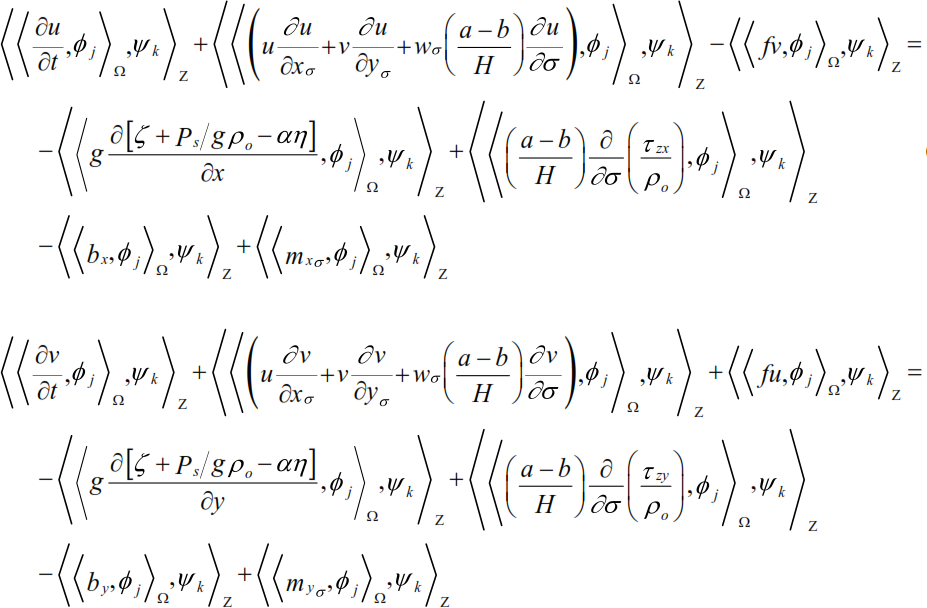
\includegraphics[width=\textwidth]{fem}
	\end{center}
\end{figure}

After applying Galerkin finite-element method, the equation above reduces to the form of the 3D momentum equations solved in ADCIRC

\begin{figure}[H]
	\begin{center}
		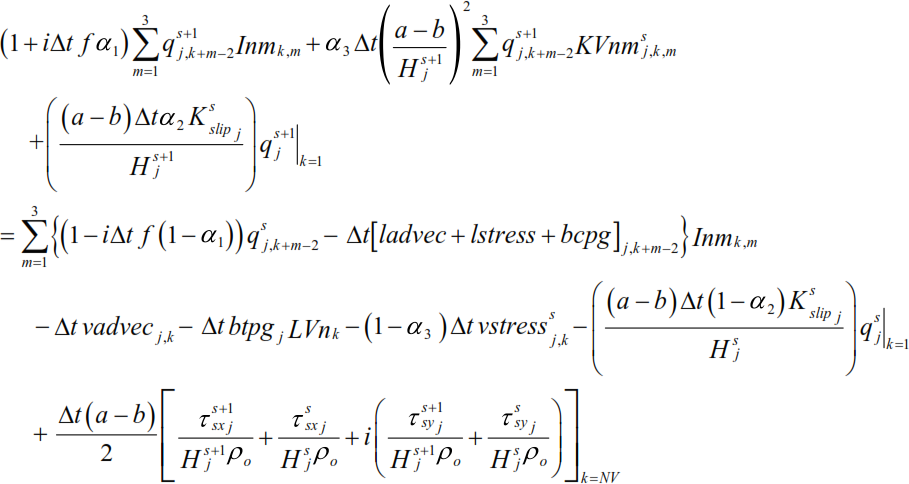
\includegraphics[width=\textwidth]{fem3}
	\end{center}
\end{figure}

\begin{figure}[H]
	\begin{center}
		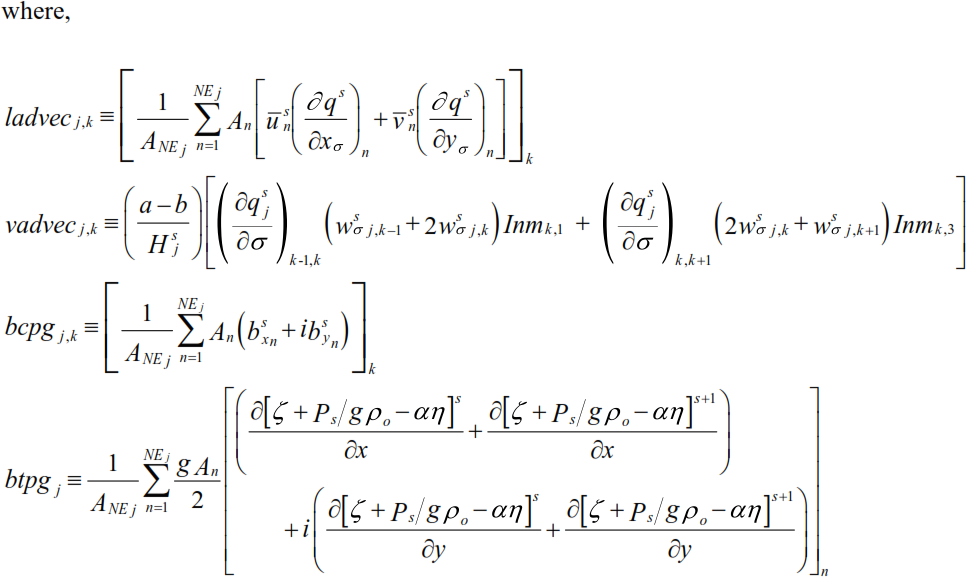
\includegraphics[width=.7\textwidth]{fem4}
		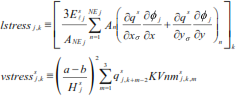
\includegraphics[width=.7\textwidth]{fem2}
	\end{center}
\end{figure}
The above equation has a tridiagonal matrix structure $Mq = F$ and this is solved by Jacobi conjugate gradient method.

\section{Methodology and Results}
Elevation was measured on three points in the domain: near Tacloban airport, near Tacloban main and an outstanding location.
\begin{figure}[H]
	\begin{center}
		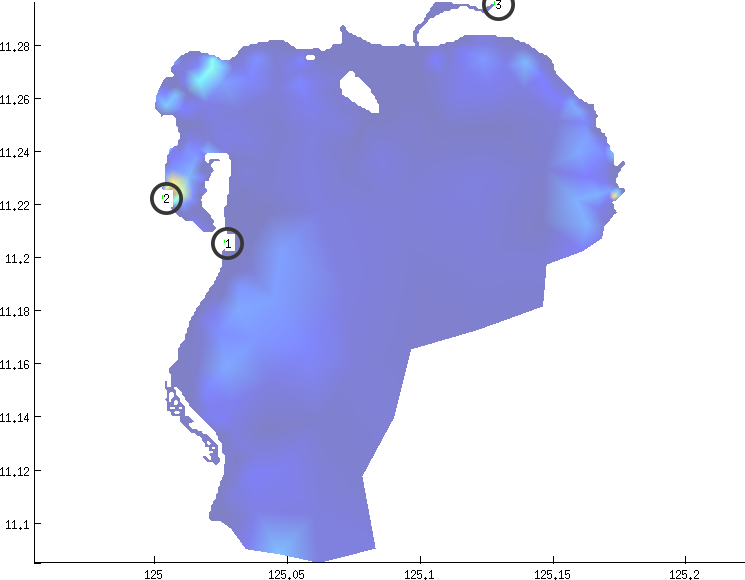
\includegraphics[width=.75\textwidth]{stations}
	\end{center}
\end{figure}

Under a normal run, the figures given below are the time-series water height of the three stations and surge height over the area on November 8, 2013:
\begin{figure}[H]
	\begin{center}
		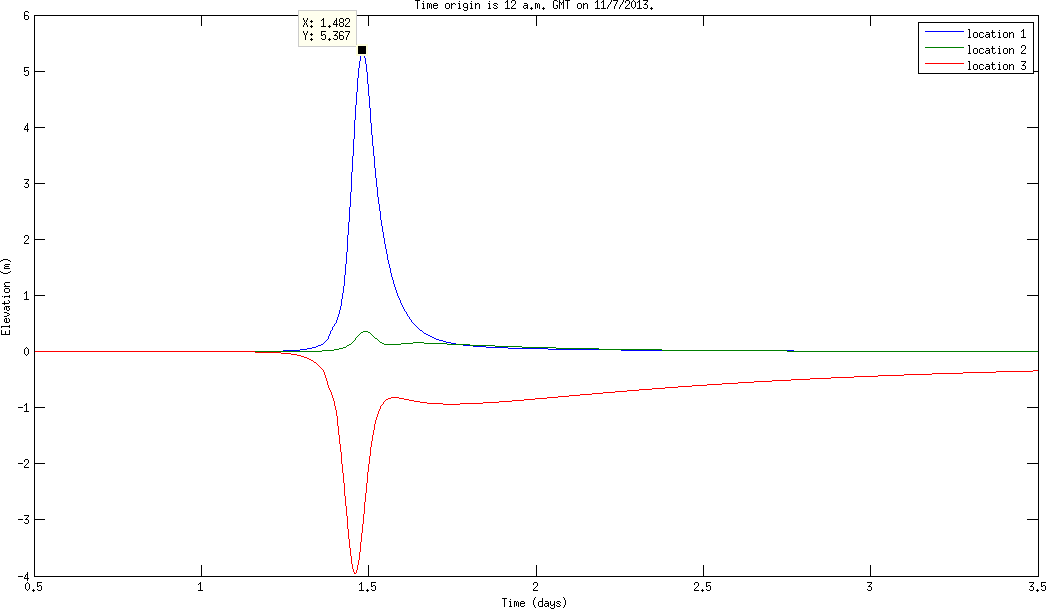
\includegraphics[width=.45\textwidth]{stoch0}
		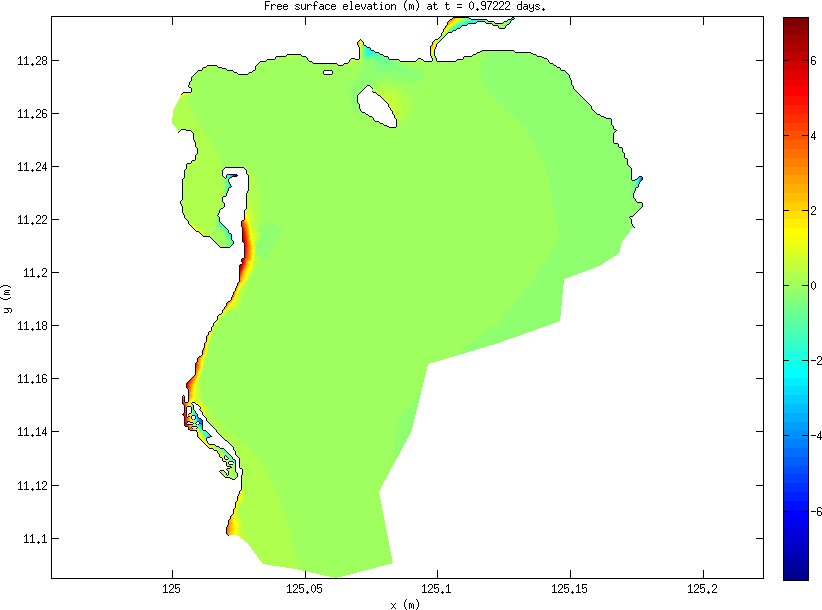
\includegraphics[width=.45\textwidth]{stoch0snap}
	\end{center}
\end{figure}

Regarding perturbation, additive noise was employed on the momentum equations in spherical coordinates [\ref{eqn:sph}] and modified the source code of ADCIRC. A random variable with uniform distribution (divided by 1000), that is $X \sim \mathcal{U}(0, 1)/1000$ are added on the right hand side of the matrix equation. Meaning, random noise was added on the force components $F$.
\begin{figure}[H]
	\begin{center}
		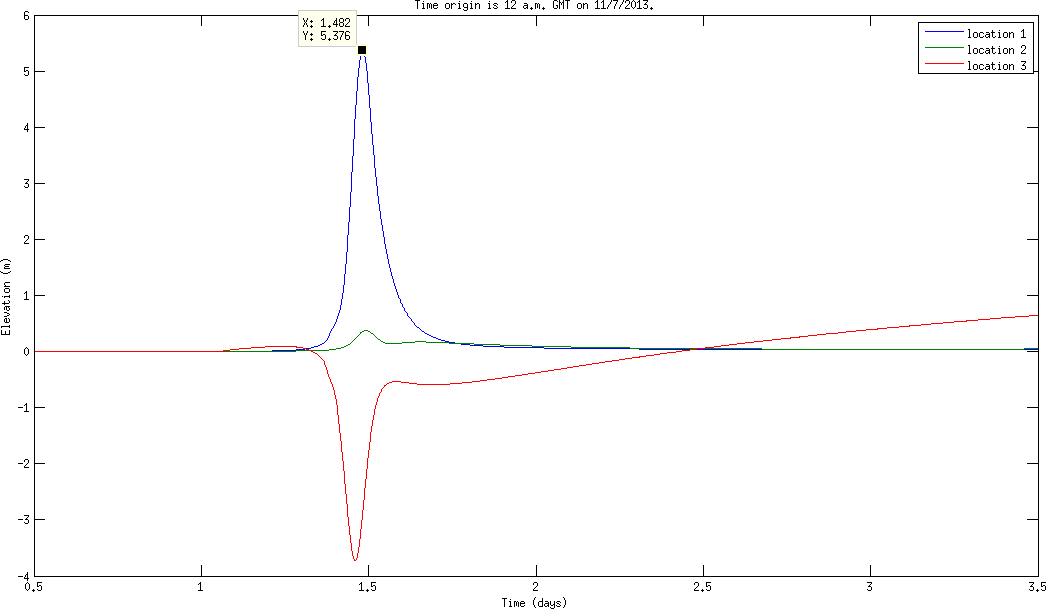
\includegraphics[width=.45\textwidth]{stoch1}
		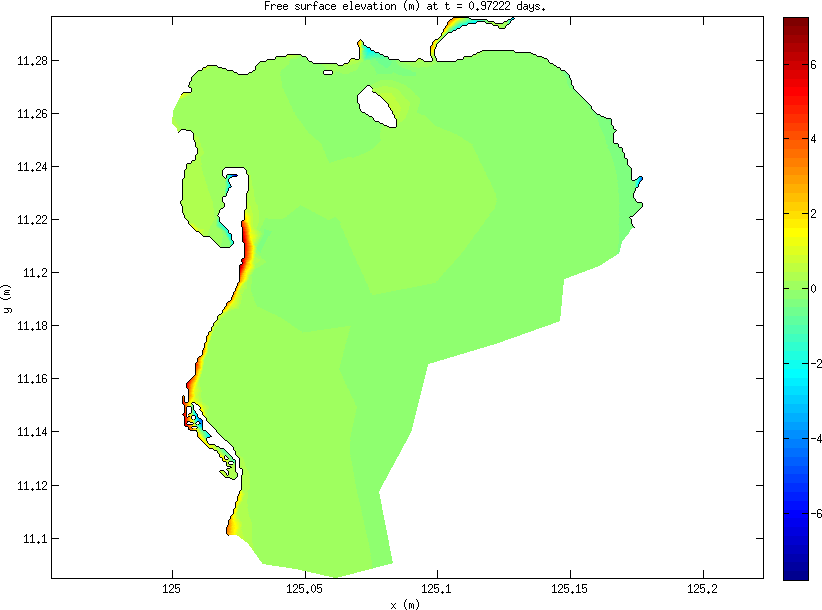
\includegraphics[width=.45\textwidth]{stoch1snap}
	\end{center}
\end{figure}

Next, a random variable with uniform distribution (divided by 10000) are added on the right hand side of the matrix equation. Uniform distribution makes the random numbers constrained within a given interval that makes the computation still stable compared to using normal distribution. The random number was divided by $10^3$ suggests that the model is very sensitive to noise and perturbations larger to those numbers lead to unstable computation.
\begin{figure}[H]
	\begin{center}
		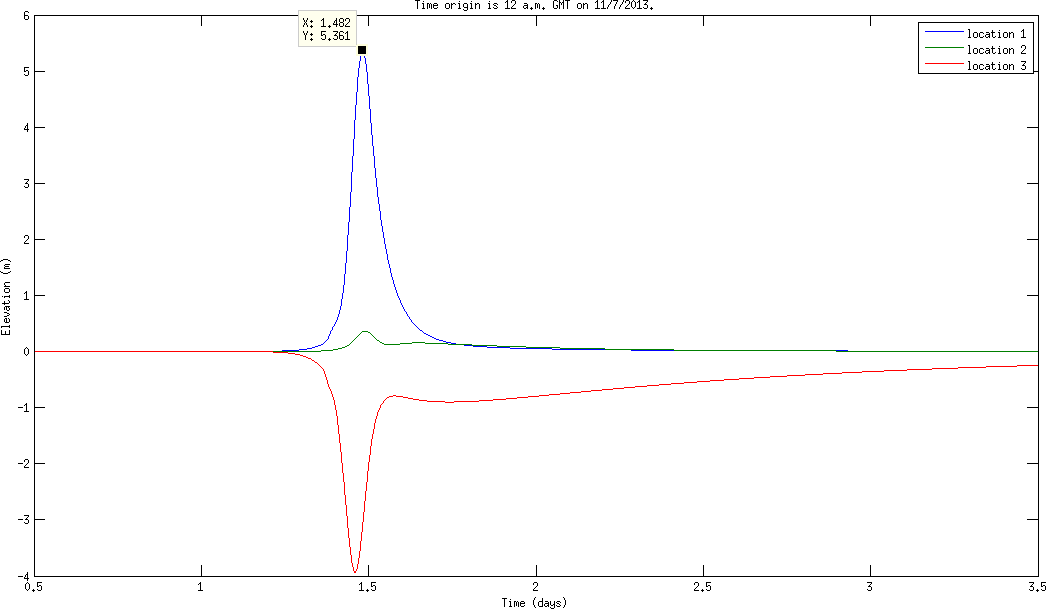
\includegraphics[width=.45\textwidth]{stoch2}
		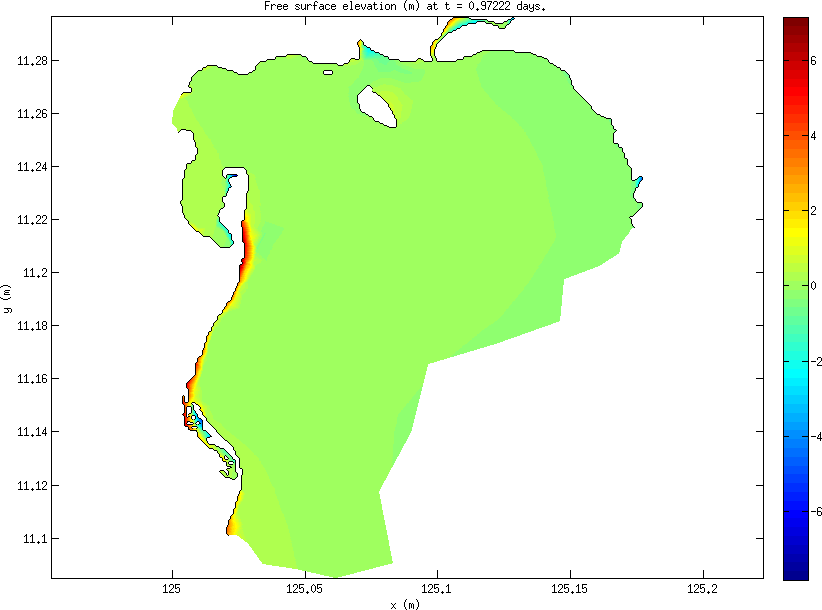
\includegraphics[width=.45\textwidth]{stoch2snap}
	\end{center}
\end{figure}


\begin{thebibliography}{9}
	\bibitem{bib:adcirc}
	R. A. Luettich, Jr., et. al. (1992), \emph{ADCIRC: An Advanced Three-Dimensional Circulation Model, Theory and Methodology}. US Army Engineer Waterways Experiment Station, Vicksburg, Mississippi.
	
	\bibitem{bib:levy}
	A. Kyprianou, \emph{Levy Processes and Continuous-State Branching Processes}. Department of Mathematical Sciences, University of Bath.
	
	\bibitem{bib:tut}
	J. R. Movellan (2011), \emph{Tutorial on Stochastic Differential Equations}. MPLab Tutorials Version 06.1
	
	\bibitem{bib:sch}
	A. Longtin (2010), \emph{Stochastic Dynamical Systems}. Scholarpedia. \url{http://www.scholarpedia.org/article/Stochastic_dynamical_systems}
	
	\bibitem{bib:app}
	V. P. Bongolan, et. al. (2008), \emph{Stochastic Terms in Boundary Conditions: Applications}. Ellis College of the New York Institute of Technology.
	
	\bibitem{bib:num}
	R. A. Luettich, Jr., et. al. (2004), \emph{Formulation and Numerical implementation of the 2D/3D ADCIRC Finite Element Model Version 44.XX}.
\end{thebibliography}

\end{document}